\documentclass[landscape,a0paper,fontscale=0.32]{baposter}

\graphicspath{{images/}}

\definecolor{dkist1}{RGB}{252,164,30}
\definecolor{dkist2}{RGB}{234,109,28}
\definecolor{dkist3}{RGB}{12,36,112}

\usepackage{fontspec}
% \setmainfont[Ligatures=TeX]{Georgia}
\setsansfont{Roboto}
\setmonofont{Source Code Pro}
\renewcommand{\familydefault}{\sfdefault}

\usepackage{minted}

\begin{document}

\begin{poster}{
 % Show grid to help with alignment
 grid=false,
 % Column spacing
 colspacing=0.7em,
 % Color style
 headerColorOne=dkist2,
 borderColor=dkist1,
 headerFontColor=dkist3,
 % Format of textbox
 textborder=faded,
 % Format of text header
 headerborder=open,
 headershape=rectangle,
 headershade=plain,
 headerheight=0.12\textheight,
 headerfont={\bfseries},
 background=none
 }
 % Eye Catcher
 {
   
\includegraphics[height=0.08\textheight]{dkistlogo.jpg}
 }
 % Title
 {\sc\Huge DKIST User Tools for Level 1 Data}
 % Authors
 {Stuart J. Mumford$^{2,1}$, Fraser Watson$^{1}$, Alisdair Davey$^{1}$\\
 {\footnotesize{1. National Solar Observatory, 2. University of Sheffield}}}
 % University logo
 {
 
\includegraphics[height=0.08\textheight]{dkistlogo.jpg}
 }
 

 
\begin{posterbox}[name=intro,column=0,row=0,span=2]{DKIST Level 1 Data}

  The DKIST Data Centre will be providing level one calibrated data for download
  by the scientific community. In addition to this a set of Python tools are
  being developed to facilitate the use of these data.

  The main features of the user tools will be:
  \begin{itemize}
  \item Dataset search.
  \item Dataset download.
  \item Loading of datasets.
  \item Providing coordinate aware representation of datasets.
  \item Enabling the use of the Scientific Python ecosystem on DKIST level 1
    data.
  \end{itemize}

  
\end{posterbox}

\begin{posterbox}[name=dataset,column=0,row=0,span=1,below=intro]{DKIST Datasets}

  The Level 1 data products provided by the DKIST data centre will be FITS files
  compliant with the FITS 4.0 specification. Each level 1 FITS file will be a
  single ``calibrated frame'', for example for the VISP slit spectrograph it
  would be a two dimensional space-wavelength array. This means every dataset
  will be comprised of many tens or hundreds of FITS files.

  The user tools expose the individual frames:

  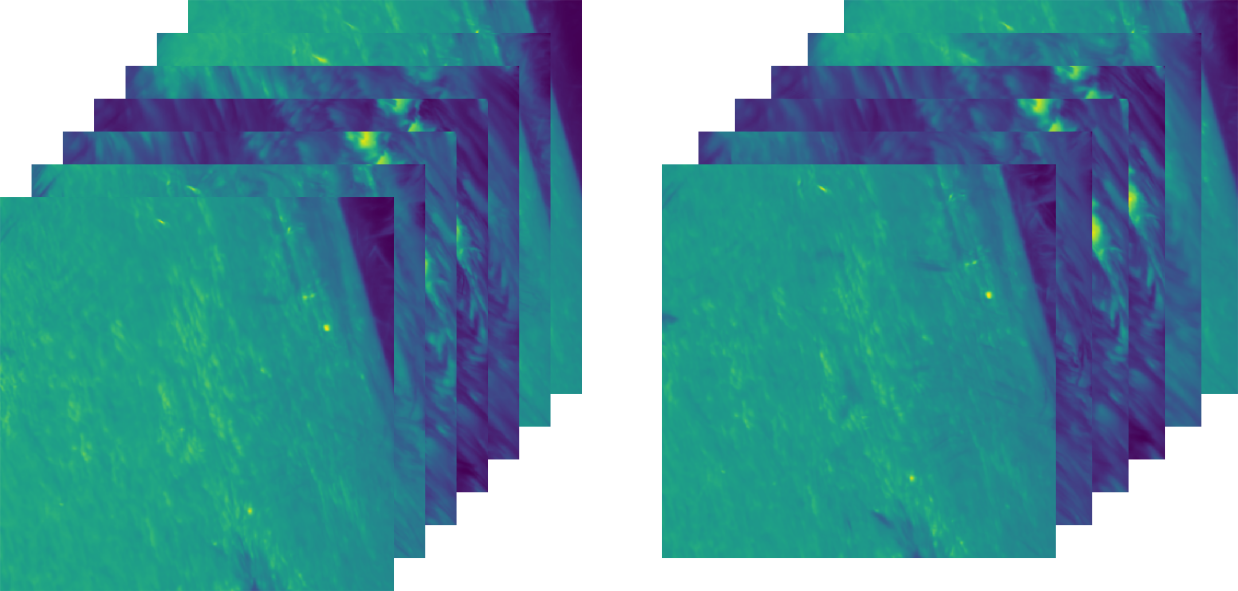
\includegraphics[width=0.98\textwidth]{sequence_of_images.png}

  as a single contiguous cube:

  \begin{center}
    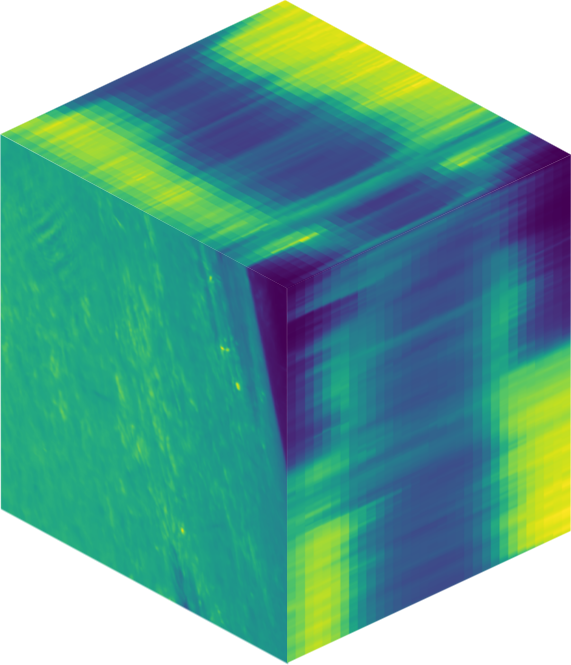
\includegraphics[width=0.49\textwidth]{cube.png}
  \end{center}

  without rewriting the data or having to open the files until the array values
  need to be read.
  
\end{posterbox}

\begin{posterbox}[name=dask,column=1,row=0,span=1,below=intro]{Dask}
  Dask is a Python library for very large datasets and parallel computation.
  While using it for DKIST data will provide users lots of potential for
  paralell computation with applications on HPC and cloud computing, the main
  motivation for using it is it's excellent support for arrays distributed over
  many files.

  The Level 1 DKIST data can construct a Dask array of all the FITS files which
  comprise a dataset by reading an Advanced Scientific Data Format (asdf) file
  which contains all the metadata for the whole dataset, but none of the arrays.
  
  \begin{minted}[xleftmargin=-15pt,fontsize=\small]{python}
    arr = arr[2:-2]
    arr = np.min(arr, axis=0)
    arr.visualize(optimize_graph=False)
  \end{minted}

  \begin{center}
    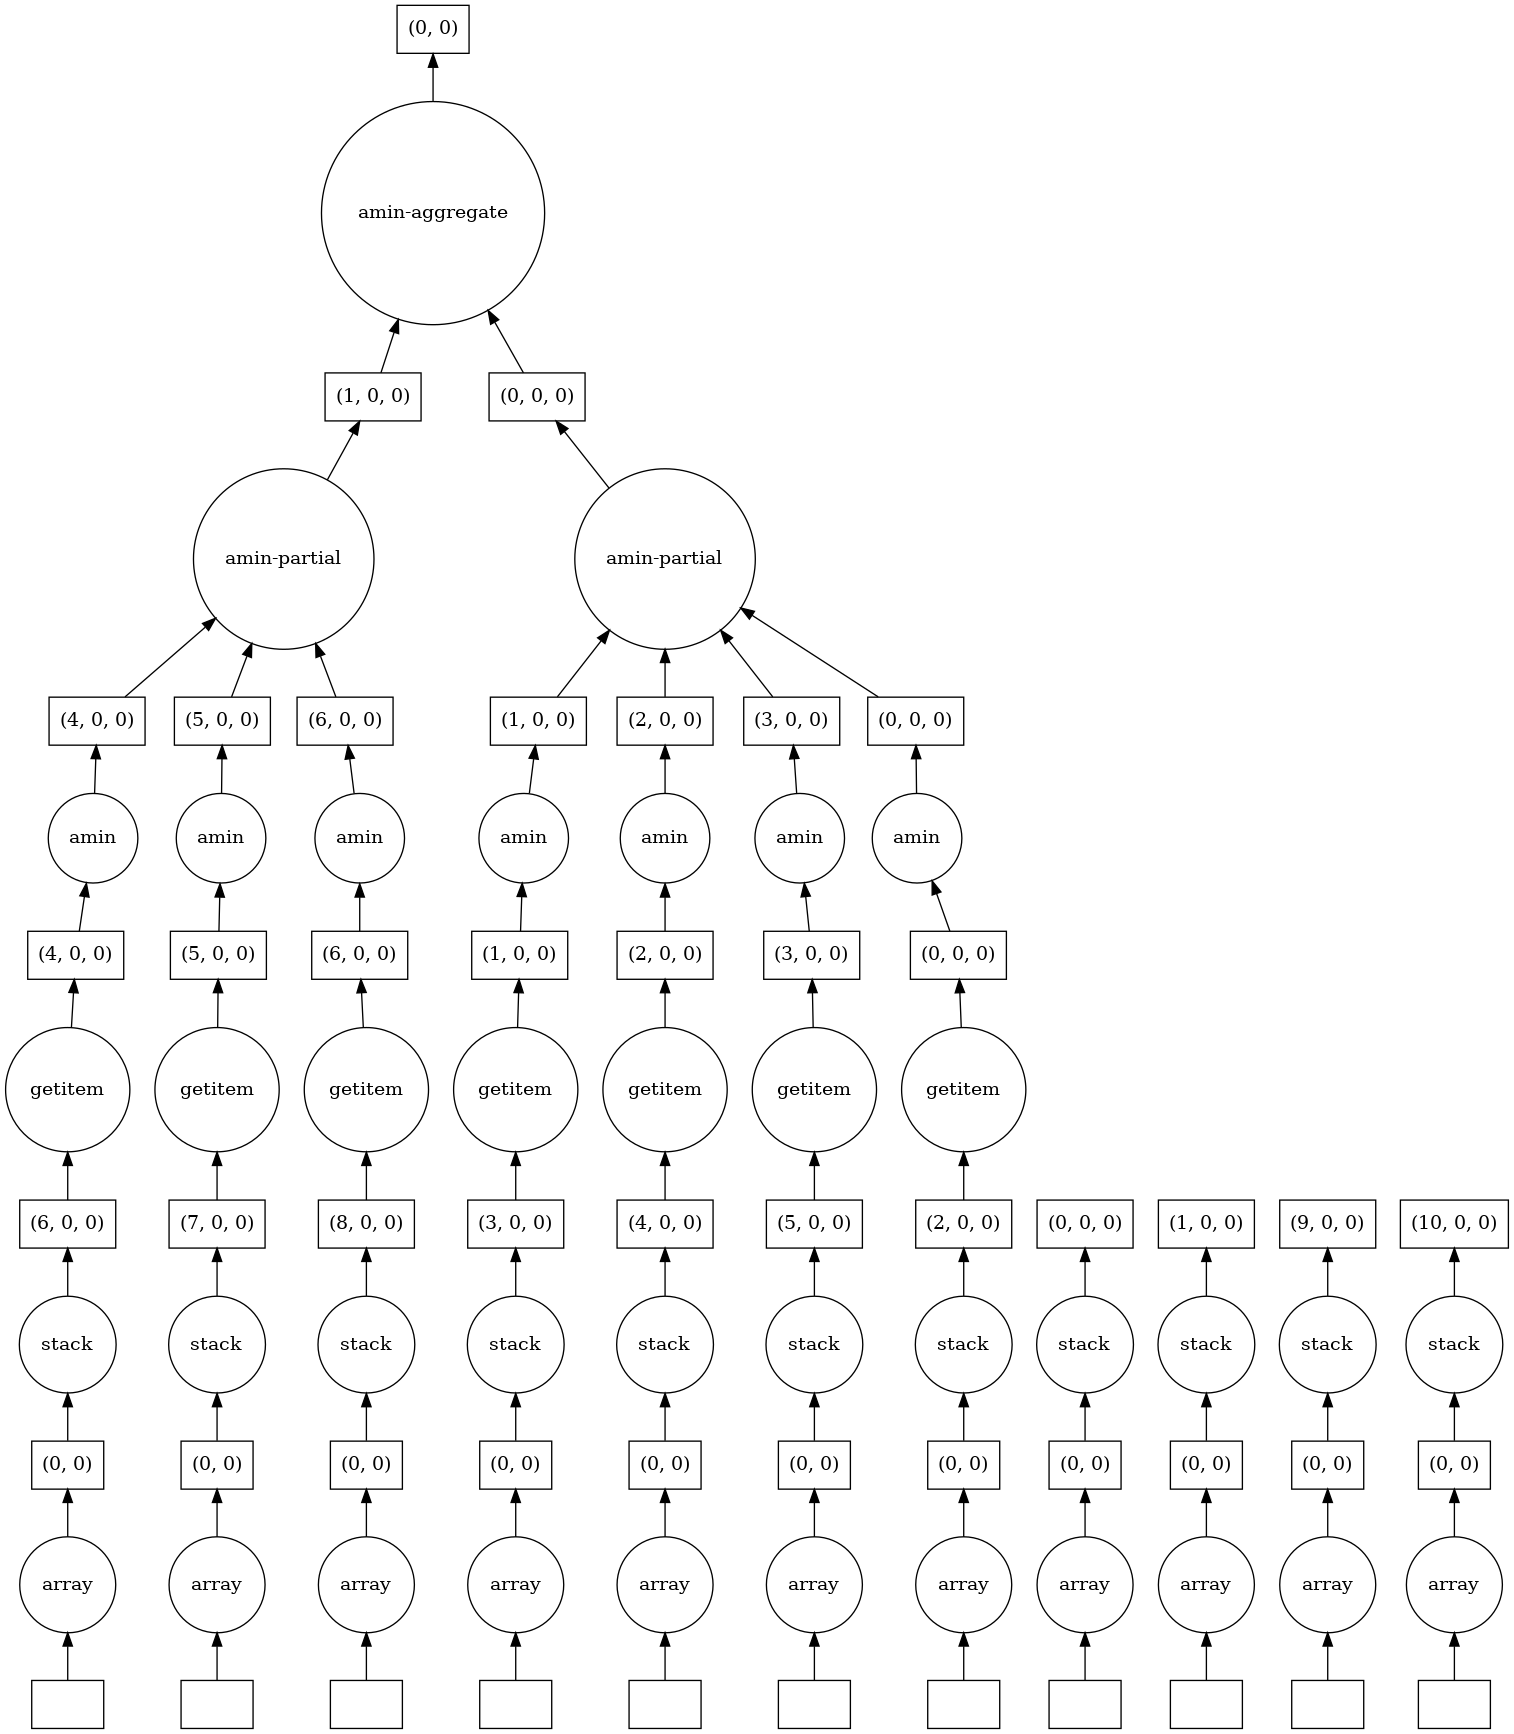
\includegraphics[width=0.6\textwidth]{mydask.png}
  \end{center}

  When doing operations on a Dask array, a graph of operations is generated, and
  only when the values of array are required is the graph executed. This means
  that complex operations can be done on a large distributed, multi-dimensional
  dataset, but then the computation can only be done on a single frame at
  visualisation or analysis time.

\end{posterbox}
 
\begin{posterbox}[name=dataset,column=2,row=0,span=2]{Loading a Dataset}
 
  \begin{minted}[xleftmargin=-15pt,fontsize=\small]{python}
   >>> from dataset import Dataset

   >>> ds = Dataset.from_directory('~/dkist_data/ae43ghig/')
   >>> ds
   <dkist.dataset.dataset.Dataset object at 0x7f3245c965c0>
   dask.array<stack, shape=(4, 128, 19, 966, 980), dtype=float32,
              chunksize=(1, 1, 1, 966, 980)>
   WCS<pixel_axes_names=(stokes, scan number, wavelength position, spatial y, spatial x),
       world_axes_names=(stokes, time, wavelength, latitude, longitude)>
  \end{minted}

\end{posterbox}

\begin{posterbox}[name=scipy,column=3,row=0,span=1,below=dataset]{Scientific Python}

  The Scientific Python ecosystem is comprised of a large number of packages
  which specialise in different functionality. The objective of the DKIST user
  tools is to enable the use of this ecosystem with DKIST data.
  
  \includegraphics[width=0.98\textwidth]{scipy-stack.png}

  The DKIST user tools uses a large number of these different packages, the main
  ones are Dask, SunPy, Astropy and matplotlib.

\end{posterbox}


\end{poster}
\end{document}